\chapter{Background: Systems Languages for Latency-Critical Software\label{chapter:background}}
% The class prints the chapter and section titles in the running head in capitals,
% where the full title of this chapter runs into the margin.
\chaptermark{Background}

\section{RAN control-plane systems and the gNB-CU-CP}\label{sec:ranarch}
The next-generation radio access network (NG-RAN) architecture disaggregates the gNB along two
independent axes. A \emph{central/distributed} split puts the higher protocol layers in a central
unit (gNB-CU) and the lower, more time-critical layers in one or more distributed units (gNB-DU)
close to the radio. A \emph{control/user-plane} split inside the central unit then separates the
control-plane function (gNB-CU-CP), which handles RRC and connection management for each
UE~\cite{3gpp38401,3gpp38300,3gpp38331}, from the user-plane function (gNB-CU-UP). The parts
communicate over standardised interfaces: NG towards the 5G core, F1 between the CU and the DU,
and E1 between the CU-CP and the CU-UP~\cite{3gpp38401,3gpp38300,3gpp38463}. Open-RAN
initiatives standardise these further so each part can come from a different vendor and run as
software on commodity hardware~\cite{polese2023oran}.

Such systems face demanding non-functional requirements: very high event rates from UE mobility
and signalling storms, strict latency bounds that the 5G service and RAN specifications quantify
as key performance indicators (KPIs)~\cite{3gpp38913,3gpp22261}, long-lived software of
continuously evolving complexity, and heavily concurrent workloads. Worst-case and tail behaviour,
not the average, determines whether deadlines are met, which motivates this thesis's focus on
predictability. Figure~\ref{fig:ngran} places the subsystem studied here, UE Context Management
(UECM), inside the gNB-CU-CP. It owns the per-UE control-plane state and mediates RRC signalling
and mobility procedures, so its correctness and timing behaviour are representative of the control
plane as a whole.

\begin{figure}[ht]
\centering
\begin{tikzpicture}[
    font=\small, >={Stealth[length=2.4mm]},
    box/.style={draw, rounded corners, minimum height=1.0cm, minimum width=1.7cm,
                align=center, fill=gray!8},
    cpbox/.style={draw, rounded corners, align=center, fill=blue!8},
    upbox/.style={draw, rounded corners, minimum width=3.1cm, minimum height=0.8cm,
                  align=center, fill=green!8},
    uecm/.style={draw, rounded corners, minimum width=2.7cm, minimum height=0.62cm,
                 fill=red!14, align=center}
  ]
  \node[box] (ue) at (0,0)   {UE};
  \node[box] (du) at (2.4,0) {gNB-DU};

  % Control plane, with UE Context Management shown nested inside it
  \node[font=\footnotesize\bfseries] (cpttl) at (7.2,1.7) {gNB-CU-CP};
  \node[uecm] (uecm) at (7.2,0.85) {UE Context\\ Management};
  \begin{scope}[on background layer]
    \node[cpbox, fit=(cpttl)(uecm), inner sep=6pt] (cp) {};
  \end{scope}
  % User plane
  \node[upbox] (up) at (7.2,-0.95) {gNB-CU-UP};

  \begin{scope}[on background layer]
    \node[draw, dashed, rounded corners, fill=gray!3,
          fit=(cp)(up), inner sep=10pt, label={[font=\footnotesize\bfseries]above:gNB-CU}] (cu) {};
  \end{scope}

  \node[box] (core) at (11.4,0) {5GC};

  \draw[<->] (ue) -- node[above,font=\scriptsize]{Uu} (du);
  \draw[<->] (du.east)         -- node[above,font=\scriptsize]{F1} (cu.west |- du);
  \draw[<->] (cu.east |- core) -- node[above,font=\scriptsize]{NG} (core.west);
  \draw[<->] (cp.south) -- node[right,font=\scriptsize]{E1} (up.north);
\end{tikzpicture}
\caption[Where the studied subsystem sits in the 5G NG-RAN]{Where the studied subsystem sits in
the 5G NG-RAN. The distributed unit (gNB-DU) and the central unit (gNB-CU), itself split into
control-plane (gNB-CU-CP) and user-plane (gNB-CU-UP) functions, connect over the standardised F1,
E1 and NG interfaces. UE Context Management (highlighted) is the per-UE control-plane state
manager this thesis reimplements and measures.\label{fig:ngran}}
\end{figure}

\section[Latency and predictability]{Latency, throughput, and predictability in real-time software}\label{sec:predictability}
Latency-critical systems are judged less by how much work they do on average than by how
\emph{predictably} they do it. Three metrics must be distinguished: \emph{throughput}, the
sustained rate of completed operations, \emph{latency}, the time one operation takes, and
\emph{jitter}, the variability of that latency. Excellent mean latency is compatible with frequent
missed deadlines, so the meaningful figures are the high-percentile \emph{tail} latencies, the
99th (p99) and 99.9th (p99.9). At the scale of a network the tail
dominates user-visible behaviour: when a single user action fans out into many internal
operations, the slowest of them sets the response time, so rare per-operation delays become
common per-request delays~\cite{dean2013tail}. Data-centre and networking software increasingly
operates where the relevant latencies are microseconds, a range in which conventional
operating-system and software overheads are no longer negligible~\cite{barroso2017microseconds}.
Fine-grained measurement shows that even at moderate utilisation, hardware, operating-system and
application-level effects such as background interference, scheduling, interrupt routing and
power-saving states inflate the tail far beyond queueing-model
predictions~\cite{li2014tales}. Figure~\ref{fig:tailconcept} sets both effects side by side.

\begin{figure}[ht]
\centering
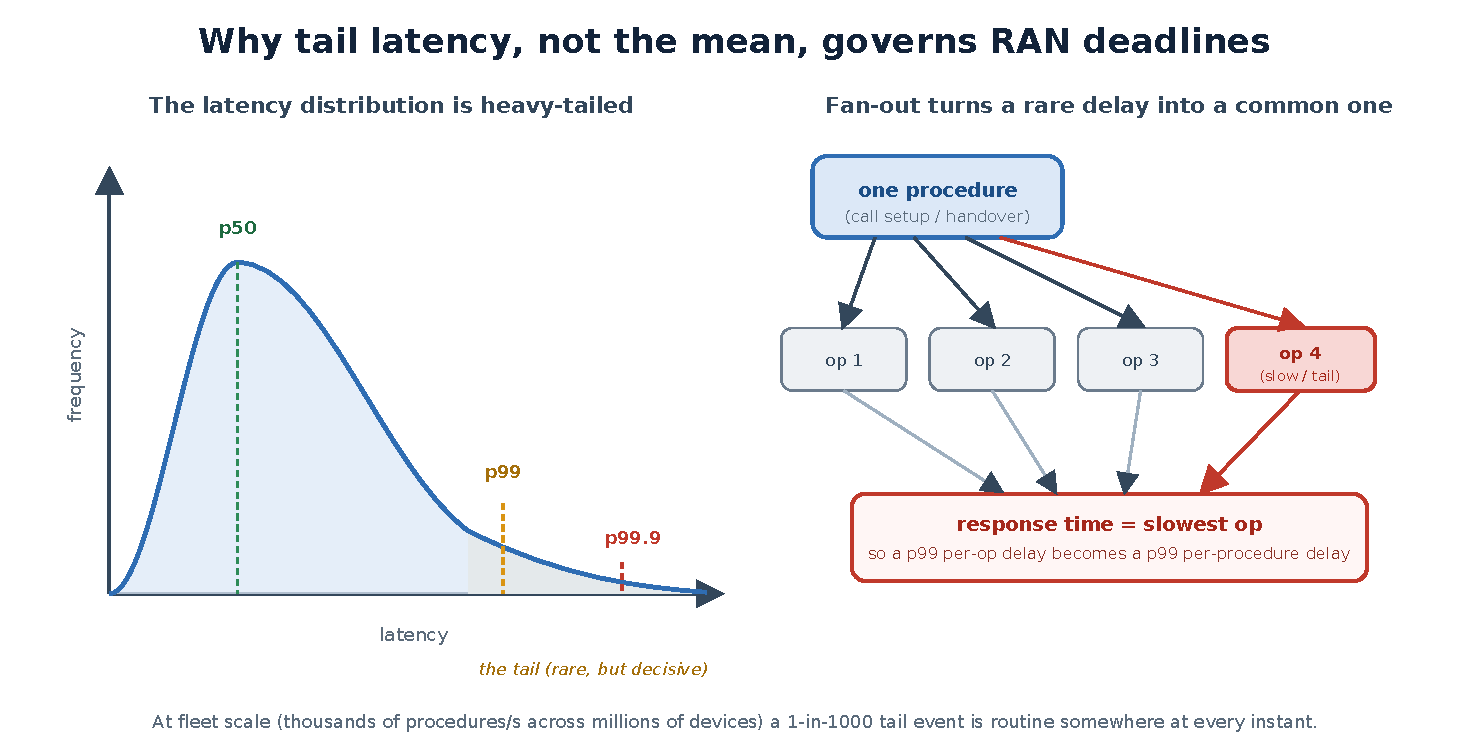
\includegraphics[width=0.78\linewidth]{diagrams/pdf/11_tail_latency_concept.pdf}
\caption[Why the tail, not the mean, governs RAN deadlines]{Why the tail, not the mean, governs
RAN deadlines. On the left, most operations finish quickly and a few take far longer, so p99 and
p99.9 sit well to the right of the median. On the right, a procedure such as a call setup
finishes only when its slowest operation does, so a delay hitting one operation in a hundred
reaches a much larger share of procedures, and at fleet scale a one-in-a-thousand delay is
happening somewhere at every instant.\label{fig:tailconcept}}
\end{figure}

Real-time systems are graded by the consequence of a missed deadline: in
\emph{hard} real-time a miss is a failure, in \emph{firm} real-time a late result is useless but
not catastrophic, and in \emph{soft} real-time a miss merely degrades quality. A RAN control
plane is best seen as soft-to-firm real-time, since an occasional late signalling response
degrades service rather than endangering it, but at fleet scale and under signalling storms such
degradations accumulate into a network-wide reliability problem. Queueing behaviour compounds
this: as offered load approaches service capacity, queueing delay grows sharply and the tail
explodes near saturation. Characterisation therefore requires driving the system not just at
nominal load but \emph{into overload}, which is why the evaluation sweeps load up to and beyond
the saturation point.

Measuring tail latency correctly is itself a pitfall. A closed-loop load generator that waits for
each response before issuing the next request suffers \emph{coordinated omission}: when the system
stalls the generator stalls with it, never recording the requests that would have arrived during
the stall, and so hides the very tail it is meant to expose (Figure~\ref{fig:coord}). Beneath
this lies a modelling distinction rather than an implementation detail. In a closed system a new
request is triggered only by the completion of a previous one, whereas in an open system arrivals
are independent of completions, and the two produce systematically different response times on the
same service process, the closed model reporting the lower
figures~\cite{schroeder2006openclosed}. Sound measurement therefore requires an open-loop model
with an intended schedule, correction for coordinated omission, high-dynamic-range (HDR) latency
histograms that keep resolution across many orders of magnitude, and statistically rigorous
reporting with repeated runs and confidence intervals, not single point
estimates~\cite{georges2007rigorous}, all of which Chapter~\ref{chapter:eval} applies.

\begin{figure}[ht]
\centering
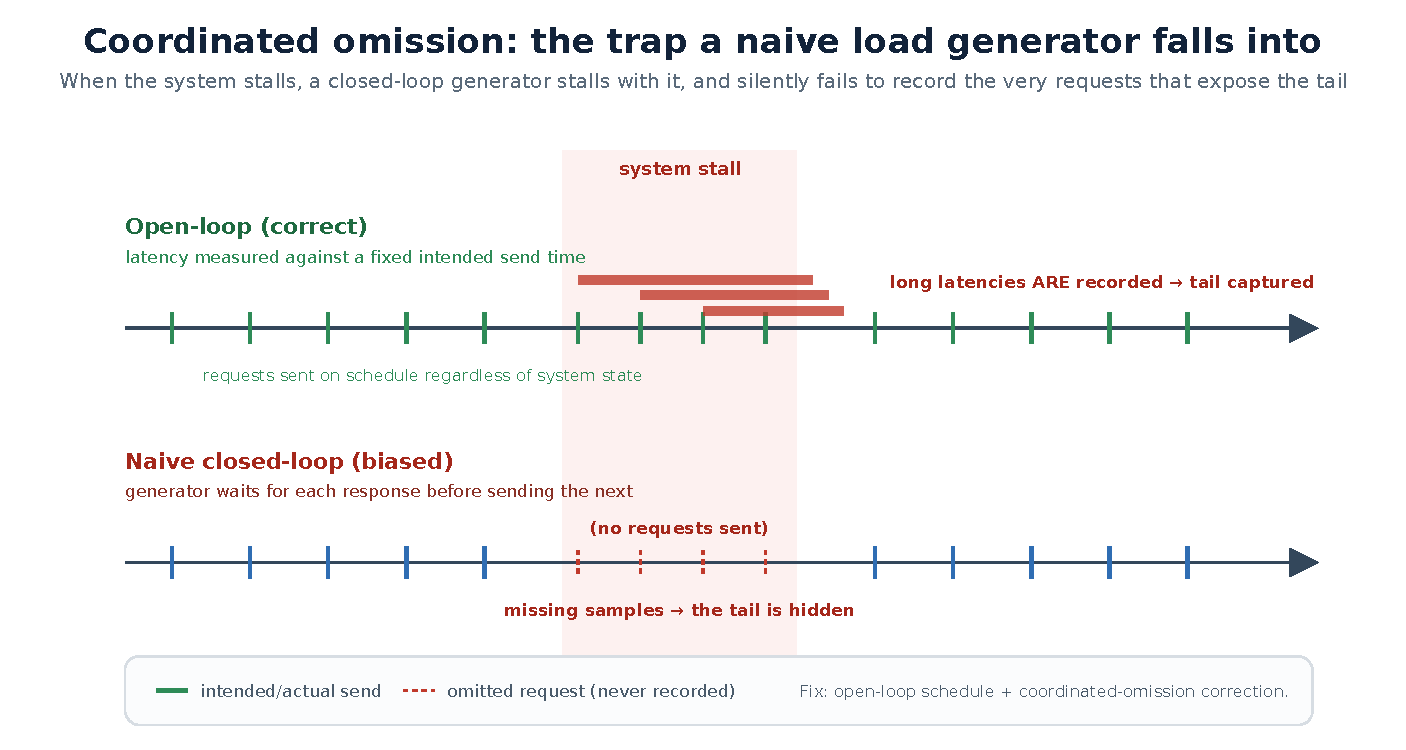
\includegraphics[width=0.78\linewidth]{diagrams/pdf/16_coordinated_omission.pdf}
\caption[Coordinated omission under open- and closed-loop load]{Coordinated omission. The
open-loop generator at the top sends on a fixed timetable even while the system is stalled and
times each request from the moment it was due, so stalled requests are recorded with their full
delay and the tail shows up. The closed-loop generator at the bottom sends the next request only
after the previous reply arrives, so when the system stalls it stops sending, the slowest requests
are never issued or measured, and the tail vanishes from the data.\label{fig:coord}}
\end{figure}

\section{C++ for latency-critical systems}\label{sec:cpplatency}
C++ is the default for RAN control-plane software with reason: zero-overhead abstractions, direct
control of memory layout and allocation, deterministic destruction through the Resource
Acquisition Is Initialization (RAII) idiom, mature compilers, libraries and profiling tools, and
no garbage collector to inject unpredictable pauses. Modern C++ (C++11 and later) adds smart
pointers (\texttt{std::unique\_ptr}, \texttt{std::shared\_ptr}) that automate ownership, move
semantics that avoid needless copies, and a formal memory model with \texttt{std::atomic} for
lock-based and lock-free concurrency. Fast and, with discipline, reasonably safe systems code is
the result.

What the compiler does not do is enforce that safety. RAII and smart pointers reduce lifetime
errors without eliminating them: a raw pointer or reference can outlive its referent, a container
mutation can invalidate an iterator, an object can be used after being moved from, and the type
system does not stop several threads sharing and writing one mutable object. Hence the familiar
catalogue, use-after-free, double-free, buffer overflow, data races, deadlocks and iterator
invalidation, easy to introduce and expensive to find at telecom scale. Memory-corruption errors
of this kind have been a security problem for decades, and deployed mitigations remain only
partial defences~\cite{szekeres2013sok}. Industry data agree: memory safety accounts for roughly
70\,\% of the vulnerabilities reported at Microsoft~\cite{msrc2019memory}, and Google reports
Android's falling below a fifth of the platform's total by 2025 as memory-safe languages were
adopted~\cite{google2022android,vanderstoep2025android}. Chapter~\ref{chapter:context} develops
the catalogue that the fault-injection study of Chapter~\ref{chapter:eval} then injects.

Mitigation rests on tooling rather than language guarantees, and tooling is partial by
construction. AddressSanitizer (ASan), ThreadSanitizer (TSan) and UndefinedBehaviorSanitizer
(UBSan) catch many errors, but only on paths a test executes with the right inputs, and their
runtime and memory overheads rule them out of production. TSan sees only the data races a run
happens to take, so one needing a rare interleaving passes unnoticed. Its deadlock detector
inherits that limit from the technique it implements, inferring deadlock potentials from a single
trace's lock-acquisition graph~\cite{bensalem2005deadlock}, and ships as an experimental component
covering only the Portable Operating System Interface (POSIX) mutex
families~\cite{tsandeadlock}. Static analysers suffer false negatives and cannot reason about the
whole program. Detection is therefore best-effort and after the fact, exactly what a language with
compile-time guarantees changes.

The language is not standing still. Since 2023 the standards committee has pursued
\emph{profiles}, named rule sets for type, bounds, lifetime and arithmetic safety that a
conforming implementation must enforce wherever they are enabled~\cite{sutter2025profiles}, in
preference to \emph{Safe C++}, a proposed safe subset with borrow checking and its own standard
library, Rust's model expressed in C++~\cite{baxter2024safecpp}. The comparison drawn here
nonetheless stays live. Profiles are not yet standardised, and in January 2026 their own authors
were still calling for implementations and treating the design of the initial profiles as work to
be done~\cite{vandevoorde2026profiles}. The concurrency profile, the one that would bear on the
defect classes catalogued in Chapter~\ref{chapter:context}, sits after that initial set rather
than in it: ``more profiles should be defined and implemented, notably a concurrency
profile''~\cite{vandevoorde2026profiles}. A rule enforced only when switched on is also a
different kind of thing from a property the type system carries unconditionally, the more so
where enforcement is a run-time check and not a compile-time rejection. The implementations
compared here are therefore built against C++23 as specified and shipped, and
Section~\ref{sec:threats} records what that pins the comparison to.

\section{The Rust ownership and safety model}
Rust enforces memory safety and data-race freedom at compile time through ownership and
borrowing~\cite{klabnik2023rust}, with modern tooling in Cargo and integrated testing. The type
system statically forbids mutation of shared state and confines the unavoidable exceptions to
\texttt{unsafe} code kept behind safe APIs~\cite{jung2021safe}.

The guarantees rest on more than assertion. RustBelt established the soundness of the language's
safe fragment formally, including the role of \texttt{unsafe} as an explicitly marked escape
hatch~\cite{jung2018rustbelt}, and the aliasing discipline even \texttt{unsafe} code must respect
has a precise operational semantics~\cite{jung2020stacked}. Practice matches: real codebases use
\texttt{unsafe} sparingly and in localised ways~\cite{qin2020rust,astrauskas2020unsafe}, and of
all Rust memory-safety entries in the Common Vulnerabilities and Exposures (CVE) list, every one
but a single compiler bug involved \texttt{unsafe} code~\cite{xu2021rustcve}. Unsafety does
propagate through dependencies, though. Fewer than a third of libraries use \texttt{unsafe}
directly, yet a much larger fraction cannot be fully statically checked because it hides
somewhere in their call chain~\cite{evans2020rust}, a further argument for the
\texttt{unsafe}-free core this thesis keeps.

One property matters most in a latency-critical setting: safety comes from the type system and
the borrow checker rather than from runtime instrumentation, and is intended to be
\emph{zero-cost}. Systems research argues Rust attains it without the overhead of garbage
collection or runtime checks, and even enables efficiency techniques impractical in
C~\cite{balasubramanian2017rust}. Whether that claim holds for a telecom control-plane workload
is what this thesis evaluates. The borrow checker also rejects the use-after-free sketched in the
introduction: a program that frees a context while a reference to it is still live does not
build. Figure~\ref{fig:borrowuaf} puts that defect in its UE Context Management form beside the
C++ version.

\begin{figure}[ht]
\centering
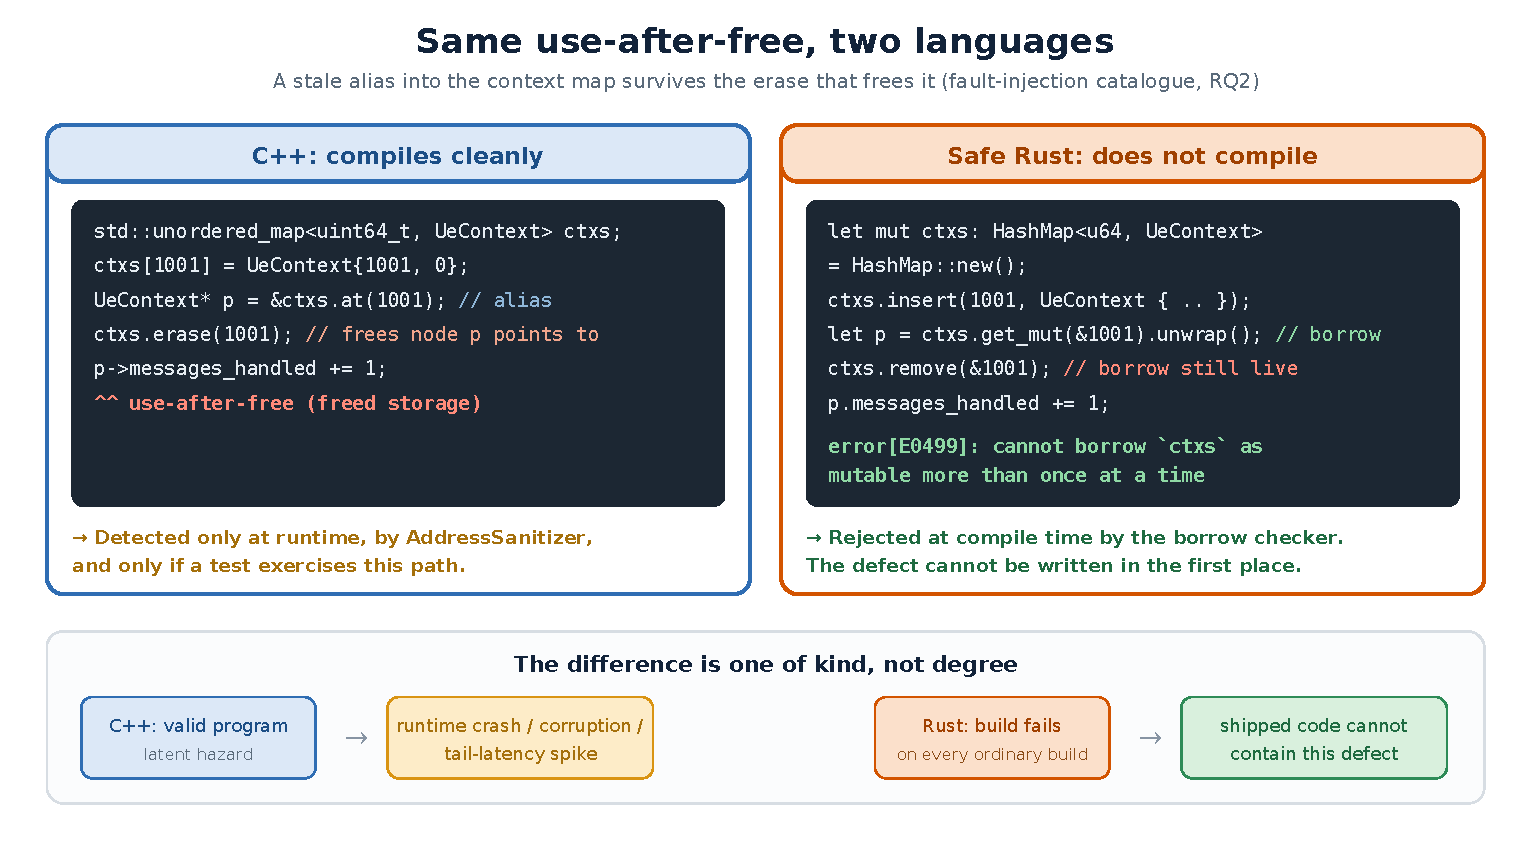
\includegraphics[width=0.78\linewidth]{diagrams/pdf/08_borrow_checker_uaf.pdf}
\caption[The same use-after-free in C++ and in safe Rust]{The same use-after-free defect in C++
and in safe Rust. The stale alias into the context map survives the
\texttt{erase}/\texttt{remove} that frees it: in C++ this compiles and is caught only at runtime,
and only under a sanitiser on a path a test exercises, whereas in safe Rust the borrow checker
rejects it at compile time (\texttt{E0499}), so the defect cannot be written at all. The
difference is one of kind, not degree.\label{fig:borrowuaf}}
\end{figure}

The discipline extends to concurrency through the \texttt{Send} and \texttt{Sync} marker traits:
a value may cross a thread boundary only if its type is \texttt{Send}, and may be shared by
reference across threads only if it is \texttt{Sync}, so sharing a value that permits
unsynchronised mutation is a compile error rather than a latent race. This is the property Rust
markets as ``fearless concurrency.'' Error handling is likewise explicit, fallible operations
returning a \texttt{Result} the caller must handle instead of raising an exception that unwinds
through hidden control flow, so the cost of the failure path stays visible, which matters in code
judged by its tail.

Rust is not the only memory-safe language, and the reason for comparing against C++ rather than a
managed runtime belongs with this model. Java, C\# and Go achieve memory safety through a runtime
and garbage collection, an excellent trade for much software and a poor one for a
tail-latency-critical control plane: collection pauses are a recognised source of tail latency in
large systems~\cite{dean2013tail}, and a managed runtime surrenders the control over memory
layout and scheduling this domain relies on. C is as memory-unsafe as C++ with fewer abstractions
for building large systems. Rust is the first widely supported language to combine compile-time
memory and thread safety with no garbage collector and throughput and memory use alongside C and
C++~\cite{balasubramanian2017rust,jung2021safe,bugden2022rust}, so managed languages are out of
scope and the meaningful comparison is C++ against Rust.

Table~\ref{tab:langmodel} sets the mechanisms side by side. Its organising distinction is not
which hazards each language names, since both name much the same ones, but \emph{when} and
\emph{by what} each is ruled out, and the last two rows mark where the answer stops being ``by
the compiler'' for either of them.

\begin{table}[H]
\centering
\small
\caption[How each language enforces the properties measured here]{How each language enforces the
properties this thesis measures. The rows above the rule are the ones on which the two differ in
kind rather than in degree: a compiler that rejects a program rules the defect out of every
execution of it, whereas a sanitiser rules it out only of the executions an instrumented test
happens to take. The rows below the rule are the boundary developed in
Chapter~\ref{chapter:context} and measured in Chapter~\ref{chapter:eval}, where neither language
offers a static guarantee.\label{tab:langmodel}}
\renewcommand{\arraystretch}{1.2}
\begin{tabular}{@{}R{0.20\linewidth} R{0.36\linewidth} R{0.36\linewidth}@{}}
\hline\hline
Concern & Modern C++ & Rust \\
\hline
Object lifetime & RAII and smart pointers, applied by convention. A raw pointer or reference may outlive its referent & Ownership: each value has one owner and is dropped exactly once \\
Aliasing & Unrestricted: any number of mutable aliases may coexist & Borrowing: either one mutable reference or many shared ones, never both \\
Bounds & Unchecked on \texttt{operator[]}, checked only through \texttt{at()} & Checked by default, elided where the index can be proved in range \\
Thread safety & Not expressed in the type system: sharing a mutable object across threads compiles & \texttt{Send} and \texttt{Sync} marker traits. Unsynchronised sharing is a type error \\
Error signalling & Exceptions or error codes: the failure path can be invisible at the call site & \texttt{Result} values the caller must handle. The failure path is explicit \\
Escape hatch & The whole language & \texttt{unsafe} blocks, delimited and mechanically countable \\
Stage of detection & Run time, under the right sanitiser, on a path a test exercises & Compile time, on every ordinary build, whatever the test coverage \\
\hline
Lock-acquisition order & Not checked & Not checked \\
Atomicity of a composed operation & Not checked & Not checked \\
\hline
\end{tabular}
\end{table}

\section{Concurrency models for control-plane software}
How concurrency is structured shapes both correctness and tail latency. The dominant model is
\emph{shared-memory} concurrency, threads mutating common state guarded by mutexes and atomics:
flexible, but the source of races, deadlocks, lock contention and priority inversion, with a
worst case that is hard to bound. The alternative is \emph{message-passing} or
\emph{shared-nothing} concurrency, where state is partitioned so each piece is owned by a single
thread and all interaction happens through messages, as in the actor model. It trades flexibility
for scalability and much simpler reasoning, and maps onto per-UE partitioning naturally, since
each UE's state is largely independent. The choice also moves the quantity measured here, because
thread-per-core structuring changes application tail latency on its
own~\cite{enberg2019threadpercore}, so the model is held fixed across both implementations
instead of left to each language's idiom. Figure~\ref{fig:concmodels} contrasts the two.

\begin{figure}[ht]
\centering
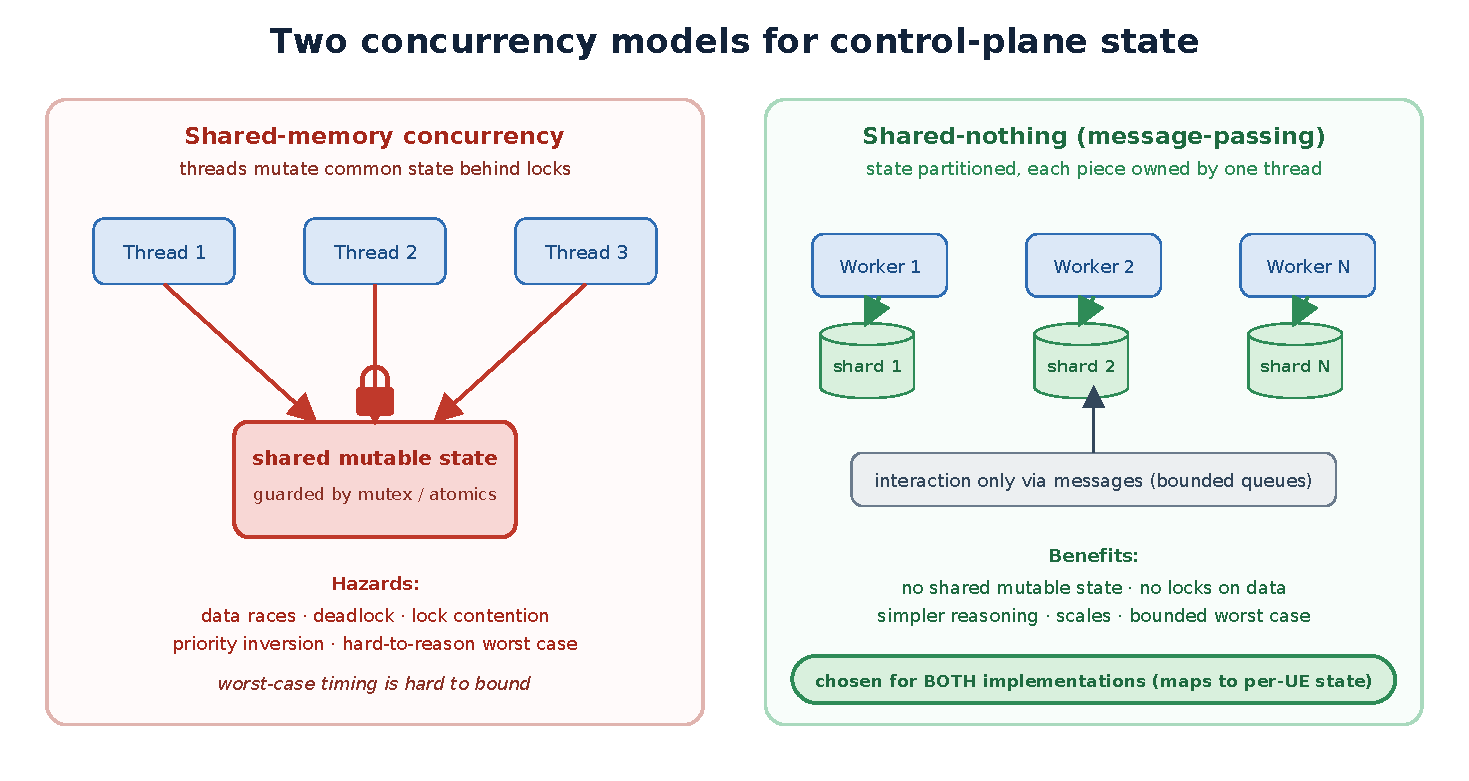
\includegraphics[width=0.78\linewidth]{diagrams/pdf/12_concurrency_models.pdf}
\caption[Two concurrency models for control-plane state]{Two concurrency models for
control-plane state. Shared-memory concurrency (left) lets threads mutate common state behind
locks and is the source of data races, deadlock and lock contention, with a worst case that is
hard to bound. Shared-nothing message-passing (right) gives each shard a single owning worker and
routes all interaction through bounded queues, which removes locks on context data and maps onto
per-UE partitioning. It is the model adopted for both implementations.\label{fig:concmodels}}
\end{figure}

A third structure, an asynchronous runtime over a work-stealing scheduler, is idiomatic in both
languages and used in neither. Its timing behaviour belongs to the runtime, not to the language
hosting it: a real-time study of asynchronous Rust finds one application meeting or missing its
deadlines depending on the runtime and thread-priority mapping it is given, and the configuration
that meets them is not the idiomatic work-stealing one~\cite{skoudlil2025asyncrust}. Adopting
such a runtime would import the variable this study exists to exclude, and
Section~\ref{sec:relatedwork} returns to a comparison in which it was not excluded.

Queueing between producers and consumers is a second, independent choice. Unbounded queues mask
overload and let latency and memory grow without limit, whereas \emph{bounded} queues, whether
they block for backpressure or shed, bound worst-case memory and make overload visible, which
predictable tail latency requires. Both choices fix the architecture used by both implementations
in Chapter~\ref{chapter:design}: a shared-nothing, thread-per-shard design in which UE state is
divided into independent slices called \emph{shards}, each owned by exactly one worker thread, so
no two threads ever touch the same context, with requests reaching a shard through a bounded
multi-producer, single-consumer queue that blocks when full.

\section{Interoperability between C++ and Rust}\label{sec:interop}
Adopting a new language in a large existing system is necessarily incremental: a Rust component
must coexist with and be callable from a substantial C++ codebase. The common denominator for
that is the C application binary interface (ABI). Rust can expose functions with
\texttt{extern "C"} linkage and hand out \emph{opaque handles} to Rust-owned objects, which C++
calls through a C header, and tooling automates parts of this: \texttt{bindgen} (Rust bindings
from C headers), \texttt{cbindgen} (C headers from Rust) and the \texttt{cxx} crate (a safer
bidirectional bridge). Interoperability is not free. Crossing the boundary steps outside the
checked language, so the seam must contain \texttt{unsafe} code, values beyond the simplest need
marshalling, and the foreign interface has to be designed deliberately. Seam size, the
\texttt{unsafe} it concentrates and per-call crossing cost are the quantities RQ4 measures in
Chapter~\ref{chapter:eval}.

One distinction bounds what those measurements can establish. Concentrating \texttt{unsafe} in
the seam says what the compiler checks, not what can happen at run time. A Rust component linked
into a C++ host shares one address space with it, so a defect on the C++ side can corrupt
Rust-owned data however much of the Rust side the borrow checker verified. This has been shown
experimentally, and the proposed remedies isolate the two heaps in hardware or in the runtime
instead of trusting the discipline of the interface~\cite{rivera2021galeed,kirth2022pkrusafe}. The
defect classes specific to Rust/C boundaries have been catalogued separately from those of either
language~\cite{li2022crosslang}, and the binding generators themselves carry
bugs~\cite{cai2026interop}. The consequence is stated once here and honoured throughout: an
\texttt{unsafe}-free core means the core's own defects are ruled out at compile time, and it does
not mean the core is protected from its host.

What has moved recently is the reach of the tooling, not the guarantee. A stateless model checker
for Rust now explores the state space of a program together with its foreign dependencies, which
puts data races arising from the interaction of the two languages within reach of a checker even
though they sit outside what the borrow checker sees~\cite{pearce2026rustmc}. That capability
arrived after the prototype measured here was built, and Chapter~\ref{chapter:conclusions} records
it as the next step for the seam.

\section{Research gap}\label{sec:gap}
The preceding sections set up the gap. The RAN control plane is a soft-to-firm real-time, highly
concurrent domain where tail behaviour under overload, not average throughput, governs the quality
the network delivers. C++ supplies the control and performance it demands but leaves whole classes
of memory and concurrency defects to best-effort detection after the fact, while Rust promises to
prevent those classes at compile time at no run-time cost and offers a credible incremental
adoption path through the C ABI.

The domain is not unstudied, and the volume of prior work is easy to underestimate because almost
none of it is indexed. At least five vendor-hosted master's theses, all carried out at Ericsson,
have compared candidate languages for RAN and telecom software. One weighs runtime cost against
development efficiency across C++, Rust and Go~\cite{karlback2021ran}. One asks whether Rust could
replace C in RAN node management~\cite{olsson2023ranmgmt}. One builds a thread-per-core packet
processor on asynchronous Rust and measures it against the Data Plane Development Kit (DPDK)
application it mirrors~\cite{olsson2023asyncpackets}. One measures median and 99th-percentile
latency for control-plane procedures across five asynchronous programming
frameworks~\cite{arvidsson2025async}. The last builds matched C++ and Rust implementations of an
Abstract Syntax Notation One (ASN.1) decompiler and compares them
statistically~\cite{emberg2023asn1}. All five are directly relevant, and two report differences
unfavourable to Rust.

Three vary the language together with the runtime and the concurrency model, so a measured
difference cannot be attributed to the language rather than to the framework built on
it~\cite{karlback2021ran,olsson2023asyncpackets,arvidsson2025async}, and their effect sizes reach
a factor of five, an indication of how much of the measurement the runtime owns. The other two
hold the design closer to fixed but report execution time and peak memory rather than tail
behaviour under rising load~\cite{olsson2023ranmgmt,emberg2023asn1}, and the closest of them,
Emberg and Wadsten, measures a stateless transformation rather than a stateful, concurrent
subsystem. Figure~\ref{fig:gapmap} sets the neighbouring studies against the properties a
controlled answer would require: each holds some of them and none holds all.

The concentration of that evidence is itself part of the gap. All five come from one vendor and
have never been tested against another organisation's software, targets or conventions, so what
is known about this question is what one company's frameworks report about it. The record on the
other side is emptier: there is no study of Rust among the indexed publications of the vendor
hosting this work, and the nearest peer-reviewed position from that side argues for making
memory-error sanitisation practical rather than replacing it with a compile-time
guarantee~\cite{gjomemo2016mesc}, the strategy this thesis tests against.
Section~\ref{sec:relatedwork} compares all five against this study.

\begin{figure}[ht]
\centering
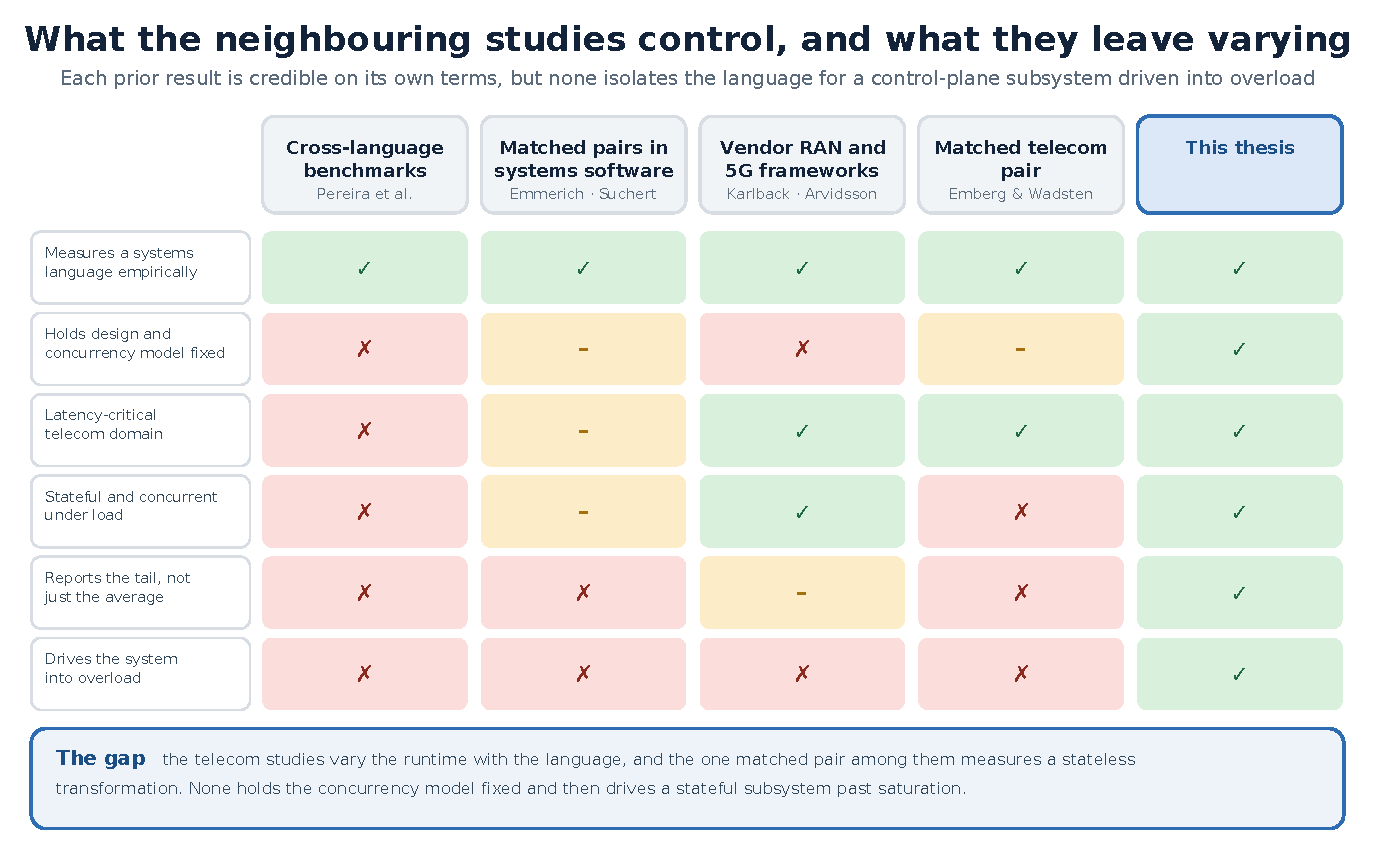
\includegraphics[width=0.78\linewidth]{diagrams/pdf/29_research_gap.pdf}
\caption[What the neighbouring studies control, and what they leave varying]{What the
neighbouring studies control, and what they leave varying. Rows are properties a controlled
answer to the research questions would need, columns are studies. The general cross-language
comparisons measure the right object in the wrong regime, averages on general-purpose workloads.
Matched pairs in systems software fix the design, but outside this domain and below saturation.
The vendor RAN and 5G framework studies reach the right domain, one reporting the tail, yet all
vary the language together with the runtime and the concurrency model. The one matched telecom
pair, Emberg and Wadsten, fixes the design but measures a stateless transformation. What this
thesis adds is design and concurrency model held fixed for a stateful, concurrent subsystem driven
past saturation. The contribution is the control, not a new measurement
technique.\label{fig:gapmap}}
\end{figure}

What is missing from the literature is therefore \emph{direct, controlled} evidence for a
representative control-plane subsystem: Whether Rust actually holds its tail latency and
predictability under overload against modern C++ \emph{when the concurrency model, algorithms,
and data structures are held fixed}, exactly which defect classes it eliminates and at what stage
the remainder are caught, what its safety model costs in throughput and resources, and what
incremental adoption costs in practice. Closing this gap is the purpose of the four research
questions, which the next chapter grounds in the specific subsystem, defect classes and timing
properties at stake, and
Chapter~\ref{chapter:methodology} sets out the methodology by which they are pursued.

